\texttt{OpenNN} has been written in ANSI C++. 
This means that the library can be built on any operating system with little effort. 
In this regard, project files of Qt Creator are included.
Nevertheless, \texttt{OpenNN} does not make use of the Qt Library. 
When working with another compiler is needed, a project for it must be created.

\subsection*{Compiling OpenNN}

Compiling \texttt{OpenNN} is easy, since it comes with project files for the latest version of Qt creator.
Qt Creator is a cross-platform IDE (integrated development environment), which is part of the Qt Project.
It can be downloaded from the following site:

\begin{flushleft}
\href{http://qt-project.org/downloads}{http://qt-project.org/downloads}
\end{flushleft}

Note that, although \texttt{OpenNN} comes with project files for Qt Creator, it does not make use of the Qt Library.
The \lstinline"opennn.pro" project file can be found in the \lstinline"opennn" folder.
To open the \texttt{OpenNN} project just double click on that file. 
A similar window than that depicted in Figure \ref{QtCreatorProject} should come up.

\begin{figure}[h!]
\begin{center}
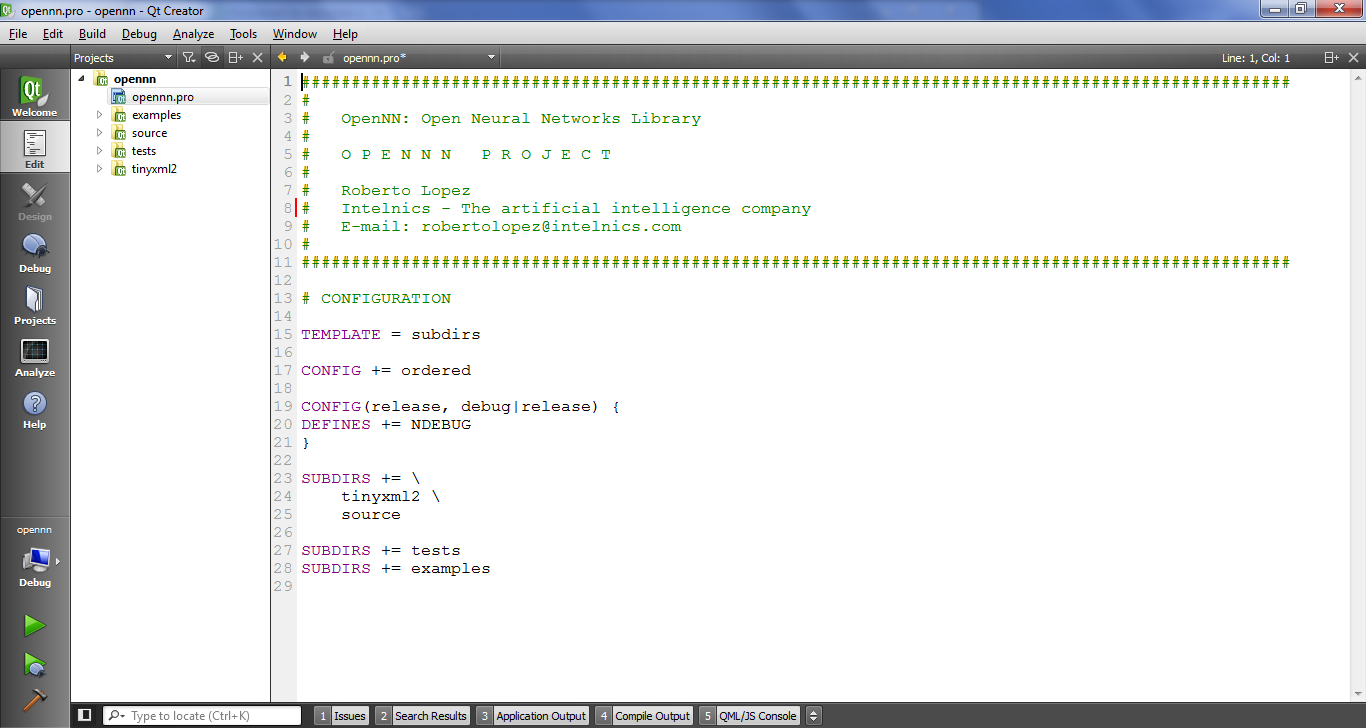
\includegraphics[width=1.0\textwidth]{preliminaries/qt_creator_project}
\caption{Qt Creator project view.}\label{QtCreatorProject}
\end{center}
\end{figure}


\subsubsection*{2. Running the test suite.}

From the \lstinline"opennn" project, select the \lstinline"test" subproject. 
That can be found at the bottom left of Qt Creator.   
Clicking on the play button or pressing \lstinline"Ctrl+R" will compile, build and run the test suite application. 
The terminal will show the following message:

\begin{lstlisting}
...

OpenNN test suite results:
Tests run: tests_run
Tests passed: tests_run
Tests failed: 0
Test OK
\end{lstlisting}

This guarantees that \texttt{OpenNN} has been compiled properly, together with all the libraries included.

\subsubsection*{3. Running an example.}

Many example subprojects are also included in the \texttt{OpenNN} distribution.
From the \lstinline"opennn" project select some example, for instance the \lstinline"simple_function_regression" subproject.  
Then run that example by clicking on the play button or pressing \lstinline"Ctrl+R".
Read the application code to see what the simple function regression example does. 
